\underbar{\textbf{\large Ejercicio 1:}} Considere el siguiente esquema:
\begin{figure}[h]
    \begin{center}
        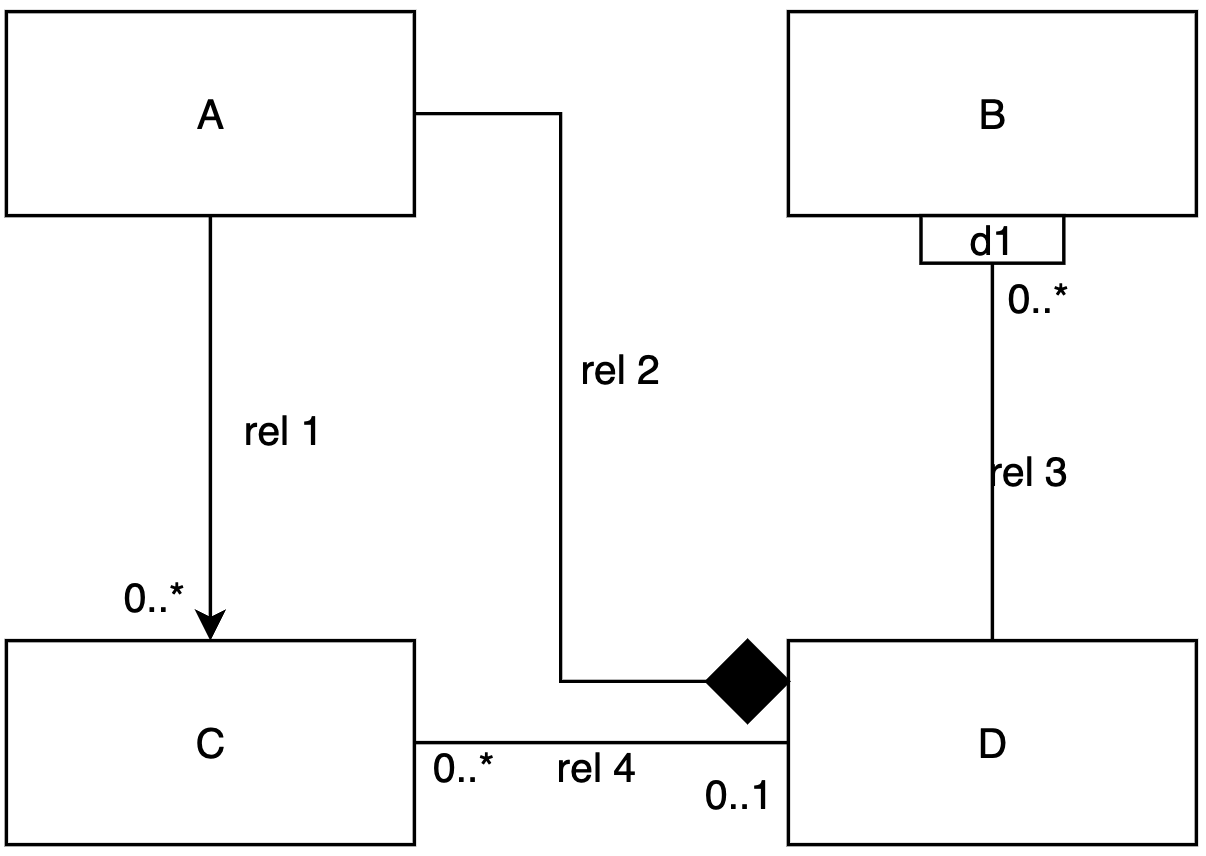
\includegraphics[width=0.45\textwidth]{assets/Junio2013_1.png}
    \end{center}
    \caption{Diagrama de clase del ejercicio}
\end{figure}
\begin{enumerate}[label = \alph*)]
    \item Escriba para cada clase los atributos extrictamente necesarios para la implementación de las relaciones en las que participan.
\begin{minted}[breaklines]{C++}
  class A{
    public:
      //Alias de la relacioncon C
      typedef std::set<C*>Cs;
      void setC(C&)noexcept;
      const Cs& getC()const noexcept;
    private:
      Cs cs_; //rel1
  };
  
  class C{  
    public:
    //como la multiplicidad es 0-1, no es necesario que para crear C exista D
      void setD(D&)noexcept;
      const D& getD()const noexcept;
    private:
      D* d_;//rel4
  };
  
  class B{
    public:
      //Alias de la relacion con D, suponemos que el tipo de dato de d1 es int
      typedef std::map<int,D*>Ds;
      void setD(D& d)noexcept;
      const Ds& getD()const noexcept;
    private:
      Ds ds_;//rel3
  };
  
  class D : private A{//rel2 como es es 1-1, herencia privada
    public:
      D(A& a):A(a){} //rel 2
      //Alias de la relacion con B
      typedef std::set<B*>Bs;
      void setB(B&)noexcept;
      const Bs& getB()const noexcept;
  
      //Alias de la relacion con C
      typedef std::set<C*>Cs;
      void setC(C&)noexcept;
      const Cs& getC()const noexcept;
  
      int clave() const noexcept{return clave_;}
    private:
      Bs bs_; //rel3
      Cs cs_; //rel4
      int clave_; //calificador
  };
\end{minted}
    \item Defina los constructores que sean oportunos para la clase C.

    C solo tendrá un constructor debido a puede que un objeto de C no esté instanciado con ningun objeto de D, por tanto, tendrá un constructor y será por omisión.
    \item Suponga que se añade un atributo de enlace x en rel1, ¿Como cambiaría los miembros de la clase A?
   
    % Al añadirse un atributo de enlace x cualquiera, ahora la \textbf{clase A} en vez de tener un conjunto de elementos de C, contendrá un diccionario clave - valor donde cada clave es un objeto de la clase C y el valor el dado por el atributo de enlace:

    Al añadirse un atributo de enlace x cualquiera, como la relación tiene una multiplicidad 1 - N, ese atributo de enlace se alamcena en la clase cuya multiplicidad es N (en este caso C) y la clase con la multiplicidad 1 (A) sigue recibiendo un conjutno de elementos de C.
    Por tanto, para cada elemento de tipo C* en dicho conjunto tendrá un atributo x (el de enlace) diferente.
\begin{minted}[breaklines]{C++}
template <typename T>
class A{
  public:
    //nueva relacion con C, donde T es el tipo del atributo de enlace
    typedef std::set<C*>Cs;
    void setC(C&);
    const Cs& getC()const noexcept;
  private:
    Cs cs_;//nueva rel1 
}
\end{minted}
No se añade nada a C de la relación, debido a que es una relación unidireccional.
\begin{minted}[breaklines]{C++}
class C{
  int x;//atributo de enlace
};
\end{minted}
\end{enumerate}

\newpage
\underbar{\textbf{\large Ejercicio 2:}} Implemente la relación rel4 del ejercicio anterior mediante una clase de asociación. Para ello:
\begin{itemize}
  \item Defina la clase con los atributos que estime oportunos y declarando métodos \texttt{asocia()} para cada sentido de la relación.
  \item Defina una función miembro que asocie un objeto C con otro de D en los supuestos:
  \begin{itemize}
    \item Cuando, en el caso de que el objeto origen ya esté asociado a otro, este objeto origen simplemente pasa a estar asociado al nuevo objeto.
    \item Cuando, en tal circunstancia, se lanza la cadena “validación de multiplicidad”.
  \end{itemize}
  \item Defina una función miembro que asocie un objeto de D con uno de C.
\end{itemize}

\begin{minted}[breaklines]{C++}
class DC{
  public:
    //Alias de las relaciones 
    typedef std::set<C*>Cs; //Conjunto de valores que tendrá la clave D
    typedef std::map<C*,D*>CDs;
    typedef std::map<D*,Cs>DCs;
    
    void asocia(D&,C&)noexcept;
    void asocia(C&,D&)noexcept;

    //observadores
    CDs getCs(D&)const noexcept; //puede haber valor de D o no
    D* getD(C&)const noexcept; //puede haber valor de C o no
  private:
    CDs directa_;
    DCs inversa_;
}
\end{minted}
\begin{minted}[breaklines]{C++}
//Implementación de los métodos
void CD::asocia(D& d, C& c)noexcept{
  
  auto i = directa_.find(&c);
  if(i != directa_.end() && i->second == &d){
    throw std::runtime_error("validación de multiplicidad"<<std::endl);
  }
  directa_[&c] = &d; //permite sobreescribir enlaces
  inversa_[&d].insert(&c);
}
void CD::asocia(C& c, D& d)noexcept{ asocia(d,c); }

DC::CDs getCs(D& d)const noexcept{
  //buscamos d está asociado
  auto i = inversa_.find(&d);
  if(i!=inversa_.end())return i->second;
  else{
    //Creamos un objeto vacio para devolverlo
    DC::Cs vacio;
    return vacio;
  }
}
D* getD(C& c)const noexcept{
  //buscamos si el objeto c está asociado
  auto i = directa_.find(&c);
  if(i!=directa_.end()) return i->second;
  else return nullptr; //si no está asociado, devolvemos un puntero nulo.
}
\end{minted}

\underbar{\textbf{\large Ejercicio 3:}} Dado el siguiente diagrama de clase:
\begin{figure}[h]
  \begin{center}
    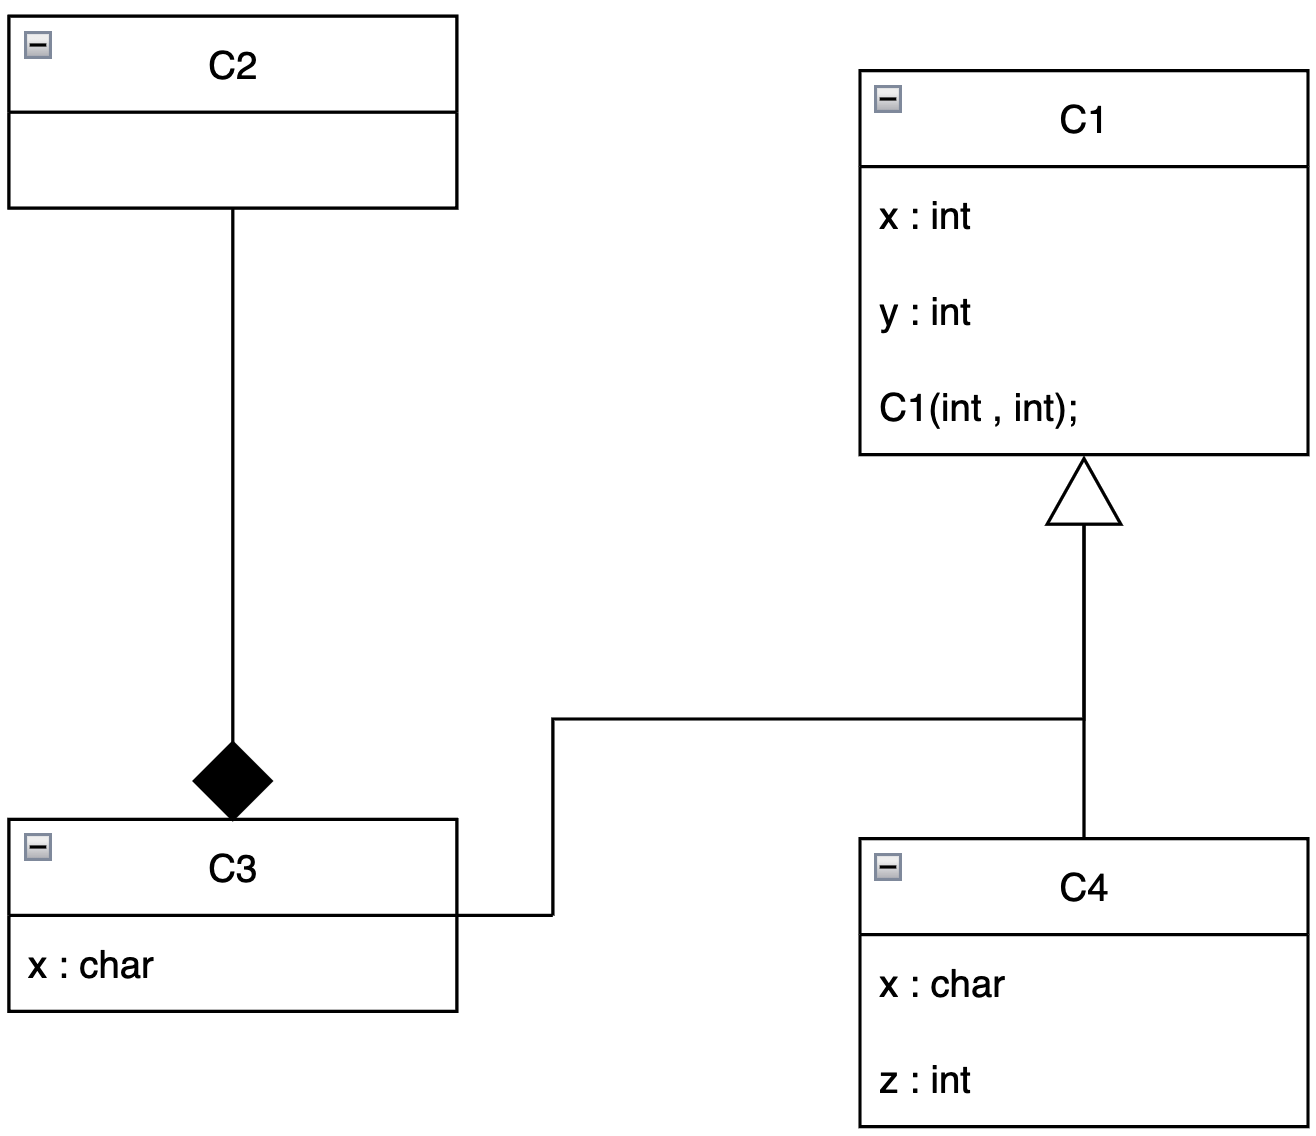
\includegraphics[width=0.66\textwidth]{assets/Junio2013_2.png}
  \end{center}
  \caption*{Diagrama de clases del ejercicio}
\end{figure}
\begin{enumerate}
  \item Defina las clases únicamente con los miembros implicados en el diagrama e implemente el constructor de la clase C3.
\begin{minted}[breaklines]{C++}
class C1{
    int x,y;
  public:
    C1(int a, int b):x(a),y(b){};
};
class C2{//..};
class C3:public C1, private C2{
    char x;
  public:
    //implementación del constructor de C3
    C3(int i, int j, char a ):C1(i,j),x(a){}
};
class C4: public C1{
    char x; int z;
  public:
    C4(char a, int b):C1(b,b)x(a),z(b){}
}
\end{minted}
\end{enumerate}
\newpage
\underbar{\textbf{\large Ejercicio 4:}} ¿Que devuelve por pantalla este programa?
\begin{center}
\begin{lstlisting}[frame = single]
using namespace std;
class B{
  public:
    void f() { cout << "f() de B" << endl; }
    virtual void g() { cout << "g() de B" << endl; }
    virtual void h() = 0;
  protected:
    int b;
};
class D1 : virtual public B{
  public:
    void f() { cout << "f() de D1" << endl; }
    virtual void g() { cout << "g() de D1" << endl; }
  protected:
    int d1;
};
class D2 : virtual public B{
  public:
    void f(int i) { cout << "f(" << i << ") de D2" << endl; }
    virtual void h() { cout << "h() de D2" << endl; }
  private:
    int d2;
};
class D3 : public D1{
  public:
    void g() { cout << "g() de D3" << endl; }
    void h() { cout << "h() de D3" << endl; }
  private:
    int d3;
};
class D4 : public D1, public  D2{
  private:
    int d4;
};
void f(B &b){
    cout << "f() externa" << endl;
    b.f();
    b.g();
    b.h();
}
\end{lstlisting}
\end{center}

\newpage
Este programa devuelve por pantalla:
\begin{center}
  \begin{lstlisting}[frame = single]
int main(){
  B b, *pb;
  D1 d1; 
  D2 d2;
  D3 d3;
  D4 d4;
  f(b); f(d1); f(d2); f(d3); f(d4);
  d4.D1::f();
  d4.f(5);
  d4.f(3.7);
  d4.g();
  d4.h();
  pb = new D4;
  pb->f();
  pb->D4::f(3);
  pb->f();
  pb->g();
  pb->h();
  delete pb;
}
  \end{lstlisting}
\end{center}

Primero de todo, vemos que en la linea 1 se quiere crear un objeto de B cuando esta es una clase abstracta y no se puede instanciar.
También vemos que la clase D1 al heredar de la clase B no está declarando el método void h() que hace que B sea abstracta, se tendría que redefinir.

\begin{minted}[breaklines]{C++}
class D1 : virtual public B{
  public:
    void f() { cout << "f() de D1" << endl; }
    virtual void g() { cout << "g() de D1" << endl; }
    virtual void h() {cout<< "h() de D1"<<endl;}
  protected:
    int d1;
};
\end{minted}

Como la clase D4 hereda publicamente de D1 y D2, al llamar al método d4.f(5) y d4.f(3.7) este serán ambigüos debido a que no sabe a cual llamar si a los de D1 o D2, lo mismo pasa con d4.h().

\begin{minted}[breaklines]{C++}
  class D4 : public D1, public  D2{
    public:
      void f(int){cout<<"f(int) de D4"<<endl;}
      void h(){cout<<"h() de D4"<<endl;}
    private:
      int d4;
  };
  \end{minted}
  
  Por último vemos que convertimos correctamente un puntero de tipo B a uno de tipo D4 y luego queremos acceder al método f() de D4, pero B no se especializa directamente en una clase D4 si no en una clase D1 o D2, por tanto, tendríamos que realizar una conversión explicita mediante dynamic\_cast.
\newpage
\begin{figure}[h]
\begin{minipage}{0.5\textwidth}
\begin{minted}[breaklines]{C++}
  int main(){
    B *pb; //desaparece el objeto b
    D1 d1; //clase bien definida
    D2 d2;
    D3 d3;
    D4 d4;
    //f(b); desaparece
    f(d1); 
    f(d2);
    f(d3);
    f(d4); 
    d4.D1::f();
    //ya no da error de ambigüedad
    d4.f(5); 
    //ya no da error de ambigüedad
    d4.f(3.7); 
    d4.g();
    d4.h();
    pb = new D4;
    pb->f();
    //tenemos que convertir el 
    //puntero pb explicitamente a un de d4.
    //pb->D4::f(3); 
    if(D4* pd4 = dynamic_cast<D4*>(pb)){
      pd4->f(3);
      delete pd4; //eliminamos el puntero usado
    }
    pb->f();
    pb->g();
    pb->h();
    pb = nullptr; //hacemos que apunte a nada antes de eliminar, para evitar errores.
    delete pb; //eliminamos el puntero
  }
\end{minted}
\end{minipage}
\hfill
\begin{minipage}{0.35\textwidth}
  \begin{lstlisting}[frame = single]
  Salida de programa corregido:
    f () externa 
    f () de B
    g() de D1
    h() de D1
    f () externa 
    f () de B
    g () de B
    h () de D2 
    f () externa 
    f () de B
    g () de D3 
    h () de D3 
    f () externa 
    f () de B
    g() de D1
    h() de D4
    f() de D1
    f(int) de D4
    f(int) de D4
    g() de D1
    h() de D4
    f () de B
    f(int) de D4
    f () de B
    g() de D1
    h() de D4
  \end{lstlisting}
\end{minipage}
\end{figure}